\section{Discussion}
\label{sec:discussion}

There are public models that work really well on your data. Using them is
important because they advance science and save energy, money and time.

Documentation is also very important. Creating standard for AI model cards could
be great for the community. This will help users and people who wants to use AI
models but which are not specialties. In WIPP we have made decision by
synthesizing the main AI Model Cards already on the market.

\def\firstellip{(1.6, 0) ellipse [x radius=2.7cm, y radius=1.5cm, rotate=50]}
\def\secondellip{(0.3, 1cm) ellipse [x radius=2.7cm, y radius=1.5cm, rotate=50]}
\def\thirdellip{(-1.6, 0) ellipse [x radius=2.7cm, y radius=1.5cm, rotate=-50]}
\def\fourthellip{(-0.3, 1cm) ellipse [x radius=2.7cm, y radius=1.5cm, rotate=-50]}

\begin{figure}[H]
\centering
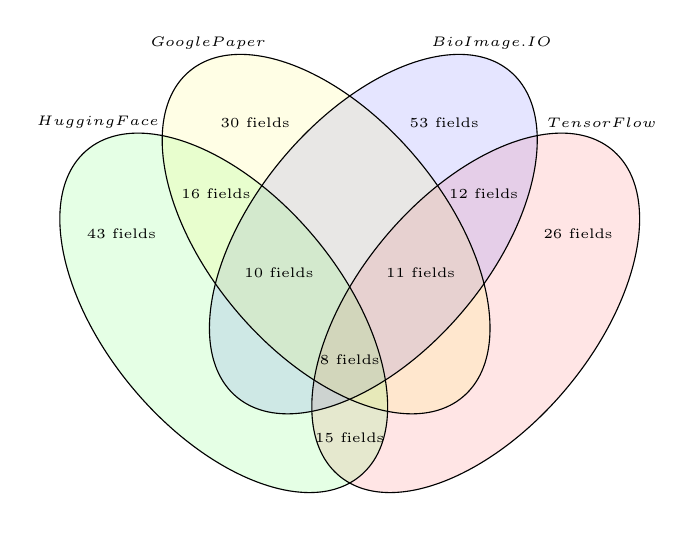
\begin{tikzpicture}

    \filldraw[fill=red,opacity=0.1] \firstellip;
    \filldraw[fill=blue,opacity=0.1] \secondellip;
    \filldraw[fill=green,opacity=0.1] \thirdellip;
    \filldraw[fill=yellow,opacity=0.1] \fourthellip;

    % TensorFlow (TF)
    \draw \firstellip node [label={[xshift=1.6cm, yshift=2.1cm] \tiny $TensorFlow$}] {};
    \draw node [label={[xshift=2.9cm, yshift=0.7cm] \tiny 26 fields}] {};

    % BioImage.IO (BI.IO)
    \draw \secondellip node [label={[xshift=1.5cm, yshift=2.1cm] \tiny $BioImage.IO$}] {};
    \draw node [label={[xshift=1.2cm, yshift=2.1cm] \tiny 53 fields}] {};

    % Hugging Face (HF)
    \draw \thirdellip node [label={[xshift=-1.6cm, yshift=2.1cm] \tiny $Hugging Face$}] {};
    \draw node [label={[xshift=-2.9cm, yshift=0.7cm] \tiny 43 fields}] {};

    % Google Paper (GP)
    \draw \fourthellip node [label={[xshift=-1.5cm, yshift=2.1cm] \tiny $Google Paper$}] {};
    \draw node [label={[xshift=-1.2cm, yshift=2.1cm] \tiny 30 fields}] {};

    % 
    \draw node [ label={ [xshift=-1.7cm,  yshift=1.2cm]   \tiny 16 fields} ] {};   % HF x GP
    \draw node [ label={ [xshift=1.7cm,   yshift=1.2cm]   \tiny 12 fields} ] {};   % BI.IO x TF
    \draw node [ label={ [xshift=0cm,     yshift=-1.9cm]  \tiny 15 fields} ] {};   % HF x TF
    \draw node [ label={ [xshift=-0.9cm,  yshift=0.2cm]   \tiny 10 fields} ] {};   % BI.IO x HF x GP
    \draw node [ label={ [xshift=0.9cm,   yshift=0.2cm]   \tiny 11 fields} ] {};   % BI.IO x TF x GP
    \draw node [ label={ [xshift=0cm,     yshift=-0.9cm]  \tiny  8 fields} ] {};   % HF x GP x BI.IO x TF

\end{tikzpicture}
\caption{Common field of different AI Model Cards} \label{fig:venn}
\end{figure}

This give us 8 fields that we want to keep to be as compatible as possible with
external tools. At the end we proposed an AI model card with 14 fields. For our
needs, this works well, and we manage to retrieve all this information
automatically throughout the workflow.

\begin{figure}[H]
\centering
\begin{minted}[framesep=2mm,baselinestretch=1.2,fontsize=\footnotesize,linenos]{java}
public class AiModelCard {
    private String              version;
    private String              name;
    private Date                date;
    private String              framework;
    private Map<String, String> trainingData;
    private Map<String, String> trainingParameters;
    private String              author;
    private String              description;
    private String              citation;
    private String[]            operationType;
    private String              architecture;
    private Map<String, Float>  training;
    private Map<String, Float>  testing;
    private String              license;
}
\end{minted}
\caption{AI Model Card proposal in WIPP}
\end{figure}

This proposal is not perfect and needs refinering. The creation of a standard
would be a great opportunity for all the AI actors to think about what they
need.

There is no standard for the documentation and no standard for the usage.
Different technologies, with different repositories, with different goals make
everything complicated. For this reason it could be great to develop a standard
way to access AI models. This will allow to use more models from more different
repositories to give access to more people. For this paper we have tried to use
some repositories like below.

\begin{table}[H]
    \centering
    \caption{\label{tab:discussion}%
        Repositories not selected for this work
    }
    \begin{tabular}{lcccc}
      \toprule
      Repository & Mask Generation Model(s) \\
      \midrule
      PyTorch Hub & +50 \\
      Dinov2 & +10 \\
      Hailo.AI & 1 \\
      ModelZoo & 2 \\
      MicroSAM & +10 \\
      \bottomrule
    \end{tabular}
\end{table}

The lack of documentation, of API or of models available made it impossible to
use these repositories in WIPP. We hope to be able to integrate them into our
tool in the future.
